\section{Proof of the Theorems}
\label{section:differentiable}

The proofs of Theorems \ref{DifferentiableIsPspace} and \ref{KTimesIsCH}
proceed as follows. 
In Section~\ref{section:divp}, 
we define \emph{difference equations}, 
a discrete version of the differential equations. 
In Section~\ref{subsection: counting hierarchy}, 
we show the $\classPSPACE$- and $\classCH$-hardness of 
difference equations with certain restrictions. 
In Section~\ref{subsection: ode family}, 
we show that these classes of difference equations are simulable 
by certain families of differential equations
given by $\classC ^{(\infty, 1)}$ and $\classC ^{(\infty, k)}$ functions. 
In Section~\ref{subsection: proof of theorems}, 
we put these families of functions together into one real function
to obtain the smooth differential equations stated in the theorems. 

The idea of simulating difference equations with differential equations
is essentially from the proof of 
the Lipschitz version \cite{kawamura2010lipschitz}.
In this paper we focus on the structure of difference equations
to analyze precisely the effect of smoothness assumptions.
Consequently we show differential equations 
given by $\classC ^{(\infty, k)}$ functions
can simulate difference equations of restricted \emph{height}, 
and this leads to the proof of $\classCH$-hardness.

\subsection{Difference Equations}
\label{section:divp}

In this section, we define difference equations, 
a discrete version of differential equations,
and show the $\classPSPACE$- and $\classCH$-hardness of 
families of difference equations with height restrictions. 

Let $[n]$ denote $\{0, \dots , n-1\}$.
Let $G \colon [P] \times [Q] \times [R] \to \{-1, 0, 1\}$ and
$H \colon [P + 1] \times [Q+1] \to [R]$. 
We say that $H$ is the solution of the \emph{difference equation} given by $G$
if for all $i \in [P]$ and $T \in [Q]$ (Figure~\ref{fig:divp}), 
\begin{figure}
 \begin{center}
  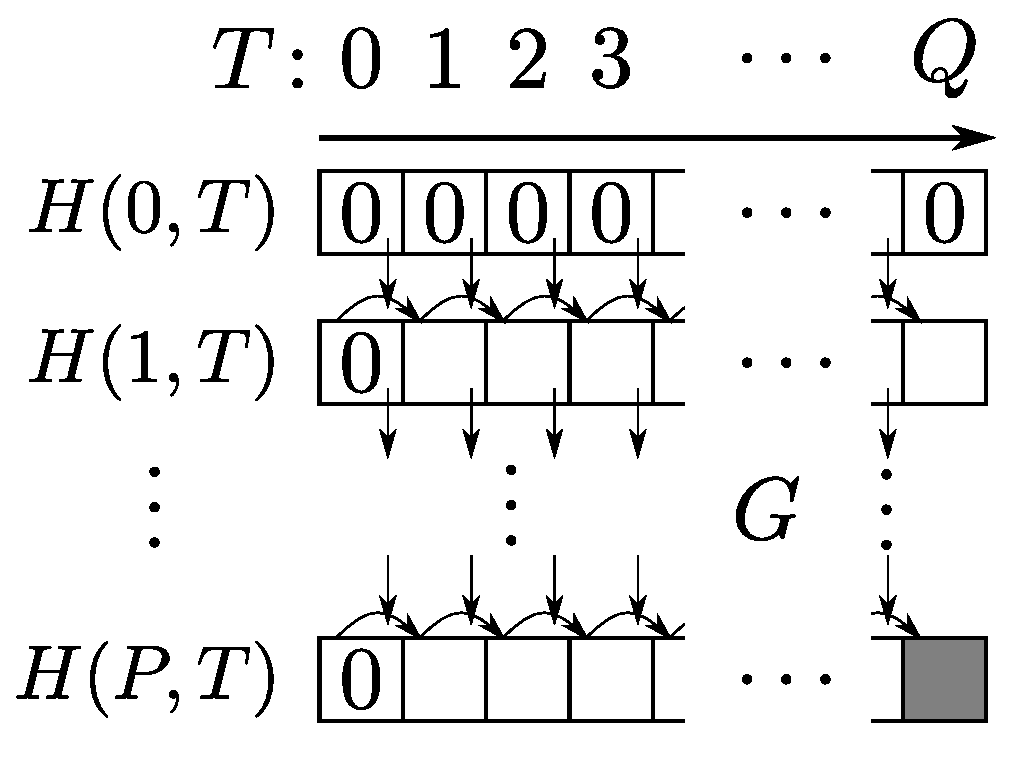
\includegraphics[height=0.15\textheight]{image/divp.eps}
 \end{center}
 \caption{The solution $H$ of the difference equation given by $G$}
 \label{fig:divp}
\end{figure}
\begin{gather}
   H(i, 0) = H(0, T) = 0, \label{eq:initial value}
\\
   H(i + 1, T + 1) - H(i+1, T) = G(i, T, H(i, T)).  \label{eq:divp}
\end{gather}
We call $P$, $Q$ and $R$ the \emph{height}, \emph{width}, \emph{cell size} of
the difference equation.
The equations \eqref{eq:initial value} and \eqref{eq:divp} are similar to 
the initial condition $h(0) = 0$ and the equation $\D h(t) = g(t, h(t))$ 
in \eqref{eq:ode}.
In Section~\ref{subsection: ode family}, we will simulate difference equations by differential equations using this similarity.

We use a family of difference equations as a computing system by
interpreting the value of the bottom right cell (the gray cell in Figure~\ref{fig:divp}) as the output. 
A family $(G_u)_u$ of functions 
$G_u \colon [P_u] \times [Q_u] \times [R_u] \to \{-1, 0, 1\}$
\emph{recognizes} a language $L$ if for each $u$,
the solution $H_u$ of the difference equation given by $G_u$ exists 
and $H_u(P_u, Q_u) = L(u)$.
A family $(G_u)_u$ is \emph{uniform} 
if the height and width and cell size of $G_u$ are polynomial-time computable from $u$
and $G_u(i, T, Y)$ is polynomial-time computable from $(u, i, T, Y)$.
Note that height, width and cell size of a uniform $G_u$ is bounded by $2^{p(|u|)}$ where $p$ is some polynomial.
A family $(G_u)_u$ has \emph{polynomial height} if the height $P_u$ is bounded by some polynomial $p(|u|)$.
A family $(G_u)_u$ has \emph{logarithmic height} if the height $P_u$ is bounded by $c \log |u| + d$ with some constants $c$ and $d$.
In terms of these definition,
\cite[Lemma 4.7]{kawamura2010lipschitz}, proved by Kawamura to show 
the $\classPSPACE$-hardness of the Lipschitz version,
can be written in the following form:
\begin{lemma}
 \label{DIVPpolyIsPSPACEhard}
 There exists a $\classPSPACE$-hard language $L$ that is recognized by some uniform family of functions with polynomial height%
 \footnote{In \cite[Lemma 4.7]{kawamura2010lipschitz}
 it is stated that the language class recognized by 
 uniform families with polynomial height coincides $\classPSPACE$.
 }.
\end{lemma}

Kawamura obtained the result in the third row in Table \ref{table:related} 
by simulating the difference equations of Lemma~\ref{DIVPpolyIsPSPACEhard}
by Lipschitz-continuous differential equations. 
Likewise, 
Theorem~\ref{DifferentiableIsPspace} follows from Lemma~\ref{DIVPpolyIsPSPACEhard},
by a modified construction that keeps 
the function in class $\classC ^{(\infty, 1)}$ 
(Sections \ref{subsection: ode family} and \ref{subsection: proof of theorems}).

We show further that $\classC ^{(\infty, k)}$ functions, for any $k$, 
can simulate difference equations restricted to have logarithmic height
(Sections \ref{subsection: ode family} and \ref{subsection: proof of theorems}).
Theorem \ref{KTimesIsCH} follows from this simulation and the following lemma.
\begin{lemma}
 \label{DIVPlogIsCHhard}
 There exists a $\classCH$-hard language $L$ such that it is recognized by some uniform family of functions with logarithmic height.
\end{lemma}

The definition of the counting hierarchy $\classCH$, 
its connection to difference equations and 
the proof of Lemma~\ref{DIVPlogIsCHhard} 
will be presented in Section~\ref{subsection: counting hierarchy}. 



\subsection{The Counting Hierarchy and Difference Equations of Logarithmic Height}
\label{subsection: counting hierarchy}

The polynomial hierarchy~$\classPH$ is defined using non-deterministic polynomial-time oracle Turing machines: 
\begin{align}
 \classSigma^p_0  &= \classP,
 &
 \classSigma^p_{n+1} &= \classNP ^{\classSigma^p_n},
 &
 \classPH &= \bigcup_n \classSigma^p_n.
\end{align}
The counting hierarchy~$\classCH$
is defined similarly
using probabilistic polynomial-time oracle Turing machines~%
\cite{wagner1986complexity,toran1991complexity}: 
\begin{align} \label{eq:CH}
 \quantC_0 \classP  &= \classP,
 &
 \quantC_{n+1} \classP &= \classPP^{\quantC_n \classP},
 &
 \classCH &= \bigcup_n \quantC_n \classP.
\end{align}
It is known that $\classPH \subseteq \classCH \subseteq \classPSPACE$, 
but we do not know whether $\classPH = \classPSPACE$.


Each level of the counting hierarchy 
has a complete problem defined as follows.
For every formula $\phi(X)$ with the list $X$ of $l$ free propositional variables,
we write 
\begin{equation}
 \quantC^m X \phi(X) 
  \longleftrightarrow 
  \sum_{X \in \{0,1\}^l} \phi(X) \ge m,
\end{equation}
where $\phi(X)$ is identified with the function 
$\phi \colon \{0,1\}^l \to \{0,1\}$
such that $\phi(X) = 1$ if and only if $\phi(X)$ is true.
This ``counting quantifier'' $\quantC ^m$ generalizes 
the usual quantifiers $\exists$ and $\forall$, 
because $\quantC^1 = \exists$ and $\quantC^{2^l} = \forall$.
For lists $X _1$, \ldots, $X _n$ of variables 
and a formula $\phi(X_1, \dots, X_n)$ with all free variables listed, 
we define
\begin{equation}
 \langle \phi(X_1, \dots, X_n), m_1, \dots, m_n \rangle \in \quantC_n B_{be}
 \longleftrightarrow
 \quantC^{m_1}{X_1} \cdots \quantC^{m_n}{X_n} \phi(X_1, \dots, X_n).
\end{equation}

\begin{lemma}[{\cite[Theorem 7]{wagner1986complexity}}] \label{lemma:CnP-complete}
 For every $n \ge 1$, 
 the problem $\quantC_n B_{be}$ is $\quantC_n\classP$-complete.
\end{lemma}

We define a problem $\quantC_{\log} B_{be}$ by
\begin{equation}
 \langle 0^{2^n}, u \rangle \in \quantC_{\log} B_{be}
 \longleftrightarrow
 u \in \quantC_n B_{be}.
\end{equation}
We show that $\quantC_{\log} B_{be}$ 
is $\classCH$-hard and recognized by a logarithmic-height uniform function family,
as required in Lemma~\ref{DIVPlogIsCHhard}. 

\begin{proof}[Lemma~\ref{DIVPlogIsCHhard}]
First we prove that $\quantC_{\log} B_{be}$ is $\classCH$-hard.
For each problem $A$ in $\classCH$, there is a constant $n$ such that $A \in \quantC_n \classP$.
From Lemma~\ref{lemma:CnP-complete}, for each $u \in \{0,1\}^*$
there is a polynomial-time function $f_n$ such that
$u \in A \leftrightarrow f_n(u) \in \quantC_n B_{be}$. So
\begin{align}
 u \in A 
 & \longleftrightarrow \langle 0^{2^n}, f_n(u) \rangle \in \quantC_{\log} B_{be}.
\end{align}
Since $\langle 0^{2^n}, f_n(\cdot) \rangle$ is polynomial time computable,
$A$ is reducible to $\quantC_{\log} B_{be}$.


Next we construct a logarithmic-height uniform function family $(G_u)_u$
recognizing $\quantC_{\log} B_{be}$.
Let $u  = \langle 0^{2^n}, 
\langle \phi(X_1, \dots, X_n), m_1, \dots, m_n \rangle \rangle$, 
where $n$, $m_1, \dots, m_n$ are nonnegative integers 
and $\phi$ is a formula. 
(If $u$ is not of this form, then $u \notin \quantC_{\log} B_{be}$.)
 
We write $l_i = |X_i|$ and $s_i = i + \sum^i_{j=1}l_j$.
For each $i \in \{0, \dots, n\}$ and
$Y_{i+1} \in \{0,1\}^{l_{i+1}}, \dots, Y_n \in \{0,1\}^{l_n}$,
we write $\phi_i(Y_{i+1}, \dots, Y_n)$ for the truth value of the subformula
$\quantC^{m_{i}}{X_i} \cdots \quantC^{m_1}{X_1} \phi(X_1, \dots, X_i, Y_{i+1}, \dots, Y_n)$,
so that $\phi_0 = \phi$ and $\phi_n() = \quantC_{\log} B_{be} (u)$.
We regard the quantifier $\quantC^m$ as a function from $\N$ to $\{0,1\}$:
\begin{equation}
 C^m(x) 
  = \begin{cases}
     1 & \text{if} \ x \ge m, \\
     0 & \text{if} \ x < m.
    \end{cases}
\end{equation}
Thus,
\begin{equation} \label{eq:phi-step}
 \phi_{i+1}(Y_{i+2}, \dots, Y_n) 
  = C^{m_{i+1}}\left(\sum_{X_{i+1} \in \{ 0,1 \} ^{l_i}}
		\phi_i(X_{i+1}, Y_{i+2}, \dots, Y_{n})\right).
\end{equation}
For $T \in \N$, we write $T_i$ for the $i$th digit of $T$ written in binary,
and $T_{[i,j]}$ for the string $T_{j-1} T_{j-2} \cdots T_{i+1} T_{i}$.

For each $(i, T, Y) \in [n+1] \times [2^{s_n}+1] \times [2^{|u|}]$,
we define $G_u (i, T, Y)$ as follows.
The first row is given by
 \begin{equation}\label{eq:def-Gu:case0}
  G_u(0,T,Y) = 
   (-1)^{T_{s_1}}\phi(T_{[1,s_1]}, T_{[s_1+1,s_2]},
    \dots, T_{[s_{n-1}+1,s_n]}), 
 \end{equation}
and for $i \neq 0$, we define 
 \begin{equation} 
  G_u(i,T,Y) = 
   \begin{cases}
    (-1)^{T_{s_{i+1}}} C^{m_i}(Y) 
    & \text{if} \ T_{[1,s_i+1]} = 10 \cdots 0, \\
    0 & \text{otherwise}.
   \end{cases} 
 \end{equation}
Define $H_u$ from $G_u$ by \eqref{eq:initial value} and \eqref{eq:divp}.

We prove by induction on $i$ that $H_u(i, T) \in [2^{l_i}]$ for all $T$, and that 
 \begin{equation} \label{eq:subformula}
  G_u(i,T,H_u(i,V)) = (-1)^{V_{s_{i+1}}} 
   \phi_i(V_{[s_i+1, s_{i+1}]}, \dots, V_{[s_{n-1}+1, s_n]})
 \end{equation}
if $V_{[1, s_i +1]} = 10 \cdots 0$ 
(otherwise it is immediate from the definition that $G_u(i, V, H_u(n, V)) = 0$).

For $i=0$, the claims follows from \eqref{eq:def-Gu:case0}.
For the induction step, assume \eqref{eq:subformula}. 
We have
 \begin{equation} \label{eq:summation}
  H_u(i+1, T) 
  = \sum_{V = 0}^{T-1} G_u(i, V, H_u(i, V)).
 \end{equation}
Since the assumption \eqref{eq:subformula} implies that flipping the bit $V_{s_{i+1}}$ of
any $V$ reverses the sign of $G_u(i, V, H_u(i, V))$,
most of the summands in \eqref{eq:summation} cancel out.
The terms that is can survive satisfy that $V_{[1, s_i+1]} = 10 \cdots 0$ and
that $V$ is between $\overline{T_{s_n} \dots T_{s_{i+1}+1} 00 \dots 0}$ and 
$\overline{T_{s_n} \dots T_{s_{i+1}+1} 01 \dots 1}$,
where we write $\overline U$ for the number represented by string $U$ in binary.
Since these terms are $0$ or $1$, $H_u(i+1, T) \in [2^{l_i}]$.
Then if $T_{[1,s_{i+1}+1]} = 10 \cdots 0$,
 \begin{equation}
  H_u(i+1, T) = \sum_{X \in \{0,1\}^{l_i}}
  \phi_i(X, T_{[s_{i+1}+1, s_{i+2}]}, \dots, T_{[s_{n-1}+1, s_n]}).
 \end{equation}
By this equation and \eqref{eq:phi-step},
 \begin{multline}
  G_u(i+1,T,H_u(i+1,T)) 
  = (-1)^{T_{s_{i+2}}} C^{m_{i+1}} (H_u(i+1, T))
  \\
  = (-1)^{T_{s_{i+2}}} \phi_{i+1}(T_{[s_{i+1}+1, s_{i+2}]}, \dots, T_{[s_{n-1}+1, s_n]}),
 \end{multline}
completing the induction steps.

By substituting $n$ for $i$ and $2^{s_n}$ for $T$ in \eqref{eq:subformula},
we get $G_u(n, 2^{s_n}, H_u(n,2^{s_n})) = \phi_n() = \quantC_{\log} B_{be}(u)$.
Hence $H_u(n+1, 2^{s_n}+1) = \quantC_{\log} B_{be}(u)$.
 
We show that $(G_u)_u$ is uniform and has logarithmic height. 
The height $n+1$, the width $2^{s_n}+1$, and the cell size $2^{|u|}$
of $G_u$ are polynomial-time computable from $u$, 
and $n+1 \le \log |0^{2^n}| + 1 \le \log|u| + 1$.
\qed
\end{proof}


The language class recognized by uniform function families with $i$ rows
contains $\quantC_i \classP$ (the $i$th level of the counting hierarchy)
and is contained in $\quantC_{i+1} \classP$.
While the class $\quantC_i \classP$ is defined by \eqref{eq:CH} using oracle Turing machines,
it is also characterized as those languages Karp-reducible to $\quantC_i B_{be}$, or 
as those accepted by a polynomial-time alternating Turing machine 
extended with ``threshold states'' and having at most $i$ alternations.
Likewise, 
the language class accepted by uniform function families of logarithmic height
coincided with languages Karp-reducible to $\quantC_{\log} B_{be}$
and with those accepted by an extended alternating Turing machine with logarithmic alternations.
Since this class contains $\classCH$,
we only state $\classCH$-hard in Lemma~\ref{KTimesFamily} and Theorem $\ref{KTimesIsCH}$,
but it is not known such class how hard the class is between $\classCH$ and $\classPSPACE$.



\subsection{Families of Real Functions Simulating Difference Equations}
\label{subsection: ode family}
We show that certain families of smooth differential equations can simulate 
$\classPSPACE$-hard or $\classCH$-hard difference equations stated in previous section.

Before stating Lemma~\ref{KTimesFamily} and Lemma~\ref{DifferentiableFamily},
we extend the definition of polynomial-time computability of real function
to families of real functions.
A machine $M$ \emph{computes} a family $(f_u)_u$ of functions $f _u \colon A \to \R$ 
indexed by strings $u$
if for any $x \in A$ and any name $\phi_x$ of $x$,
the function taking $v$ to $M ^{\phi _x} (u, v)$ is a name of $f _u (x)$.
We say a family of real functions $(f_u)_u$ is polynomial-time if there is
a polynomial-time machine computing $(f_u)_u$.

 \begin{lemma}
  \label{KTimesFamily}
  There exist a $\classCH$-hard language $L$ and a polynomial $\mu$,
  such that for any $k \ge 1$ and polynomials $\gamma$,
  there are a polynomial $\rho$ and families $(g_u)_u$, $(h_u)_u$ of real functions
  such that $(g_u)_u$ is polynomial-time computable and for any string $u$:
  \begin{enumerate}
   \item \label{enum:kf:start}
	 $g_u\colon [0,1] \times [-1,1]\to \R$, $h_u\colon [0,1] \to [-1,1]$;
   \item \label{enum:equation}
	 $h_u(0) = 0$ and $\D h_u(t) = g_u(t, h_u(t))$ for all $t \in [0,1]$;
   \item \label{enum:differentiability}
         $g_u$ is of class $\classC^{(\infty, k)}$;
   \item \label{enum:boundary}
	 $
	 \D^{(i, 0)} g_u(0,y) = \D^{(i, 0)} g_u(1,y) = 0
         $ for all $i \in \N$ and $y \in [-1,1]$;
   \item \label{enum:smooth}
	 $
	 \left|\D^{(i,j)} g_u(t,y)\right| \le 2^{\mu(i, |u|) - \gamma(|u|)}
         $ for all $i \in \N$ and $j \in \{0, \dots, k\}$;
   \item \label{enum:kf:end}
	 $h_u(1) = 2^{-\rho(|u|)} L(u)$.
  \end{enumerate}
 \end{lemma}

\begin{lemma}
 \label{DifferentiableFamily}
 There exist a $\classPSPACE$-hard language $L$ and a polynomial $\mu$,
 such that for any polynomial $\gamma$,
 there are a polynomial $\rho$ and families $(g_u)_u$, $(h_u)_u$ of real functions
 such that $(g_u)_u$ is polynomial-time computable and for any string $u$
 satisfying (\ref{enum:kf:start})--(\ref{enum:kf:end}) of Lemma~\ref{KTimesFamily} with $k = 1$.
\end{lemma}

We will prove Lemma~\ref{KTimesFamily} using Lemma~\ref{DIVPlogIsCHhard} as follows.
Let a function family $(G_u)_u$ be as in Lemma~\ref{DIVPlogIsCHhard},
and let $(H_u)_u$ be the solution of the difference equation given by $(G_u)_u$.
We construct $h_u$ and $g_u$ from $H_u$ and $G_u$ 
such that $h_u(T/2^{q(|u|)}) = \sum^{p(|u|)}_{i = 0} H_u(i, T)/B^{d_u(i)}$ for each $T = 0$, \ldots, $2^{q(|u|)}$
and $\D h_u(t) = g_u(t, h_u(t))$.
The polynomial-time computability of $(g_u)_u$ follows from that of $(G_u)_u$.
We can prove Lemma~\ref{DifferentiableFamily} from Lemma~\ref{DIVPpolyIsPSPACEhard} in the same way.

In Lemma~\ref{KTimesFamily}, 
we have the new conditions (\ref{enum:differentiability})--(\ref{enum:smooth}) 
about the smoothness and the derivatives of $g_u$ 
that were not present in \cite[Lemma 4.1]{kawamura2010lipschitz}.
To satisfy these conditions, we construct $g_u$ 
using the smooth function $f$ in following lemma.

\begin{lemma}[{\cite[Lemma 3.6]{ko1991complexity}}]
 \label{SmoothFunction}
 There exist a polynomial-time function $f \colon [0, 1] \to \R$ of class $\classC^\infty$ and a polynomial $s$ such that
  \begin{enumerate}
   \item $f(0) = 0$ and $f(1) = 1$;
   \item $\D ^n f (0) = \D ^n f (1) = 0$ for all $n \ge 1$;
   \item $f$ is strictly increasing;
   \item $\D ^n f$ is polynomial-time computable for all $n \ge 1$;
   \item \label{enum:polynomial-size}
	 $|\D^n f| \le s(n)$ for all $n \ge 1$. 
  \end{enumerate}
 \end{lemma}

Although the existence of the polynomial~$s$ satisfying the condition (\ref{enum:polynomial-size}) is not stated in \cite[Lemma 3.6]{ko1991complexity},
it can be shown easily.

We only prove Lemma~\ref{KTimesFamily} here
and omit the analogous and easier proof of Lemma~\ref{DifferentiableFamily}.

\begin{proof}[Lemma~\ref{KTimesFamily}]
Let $L$ and $(G_u)_u$ be as in Lemma~\ref{DIVPlogIsCHhard},
and let a function family $(H_u)_u$ be the solution of the difference equation given by $(G_u)_u$.

By a similar argument to the beginning of the proof of \cite[Lemma 4.1]{kawamura2010lipschitz},
we may assume that there exist polynomial-time functions $p$, $j_u$
and polynomials $q$, $r$ satisfying the following properties:
\begin{gather}
 G_u \colon [p(|u|)] \times [2^{q(|u|)}] \times [2^{r(|u|)}] \to \{-1, 0, 1\},
 \\
 H_u(i, 2^{q(|u|)}) = \begin{cases}
		       L(u) & \text{if} \ i=p(|u|), \\
		       0 & \text{if} \ i<p(|u|), 
		      \end{cases}
 \\
 G_u(i, T, Y) \neq 0 \to i = j_u(T).
\end{gather}
Since $G_u$ has logarithmic height,
there exists a polynomial $\sigma$ such that $(k+1)^{p(x)} \le \sigma(x)$


We construct the families of real functions $(g_u)_u$ and $(h_u)_u$ simulating $G _u$ and $H _u$ 
in the sense that $h_u(T/2^{q(|u|)}) = \sum^{p(|u|)}_{i = 0}H_u(i, T)/B^{d_u(i)}$, 
where the constant $B$ and the function $d_u \colon [p(|u|)+1] \to \N$ are 
defined by
  \begin{align}
   B &= 2^{\gamma(|u|) + r(|u|) + s(k) + k + 3}, 
   &
   d_u(i) &= 
   \begin{cases}
    \sigma(|u|) & \text{if} \ i=p(|u|), 
    \\
    (k+1)^i & \text{if} \ i<p(|u|).
   \end{cases}
  \end{align}
For each $(t, y) \in [0,1] \times [-1, 1]$,
there exist unique $N \in \N$, $\theta \in [0,1)$, $Y \in \Z$ and $\eta \in [-1/4, 3/4)$
such that $t = (T + \theta)2^{-q(|u|)}$ and $y = (Y + \eta)B^{-d_u(j_u(T))}$.
Using $f$ and a polynomial $s$ of Lemma~\ref{SmoothFunction},
we define 
$\delta_{u,Y} \colon [0,1] \to \R$,
$
g _u \colon [0, 1] \times [-1, 1] \to \R
$ and $
h _u \colon [0, 1] \to [-1, 1]
$ by
  \begin{align}
    \label{eq:delta}
   \delta_{u, Y} (t) &= \frac{2^{q(|u|)} \D f(\theta)}{B^{d_u(j_u(T)+1)}} 
   G_u \bigl( j_u(T), T, Y \bmod 2^{r(|u|)} \bigr),
   \\
  \label{eq:gu}
  g_u(t,y) 
  &= \begin{cases}
     \delta_{u, Y}(t)
     & \text{if} \ \eta \le \frac 1 4, 
     \\
     ( 1-f ( \frac{4\eta-1}{2})) \delta_{u, Y}(t)
     + f ( \frac{4\eta-1}{2}) \delta_{u,Y+1}(t)
     & \text{if} \ \eta > \frac 1 4,
    \end{cases}
   \\
  h_u(t) 
   &= \sum^{p(|u|)}_{i=0} \frac{H_u(i, T)}{B^{d_u(i)}}  
  + \frac{f(\theta)}{B^{d_u(j_u(T)+1)}} G_u \bigl( j_u(T), T, H_u(j_u(T), T) \bigr) .
  \label{eq:hu}
  \end{align}

We will verify that $(g_u)_u$ and $(h_u)_u$ defined above satisfy all the conditions stated in Lemma~\ref{KTimesFamily}.
Polynomial-time computability of $(g_u)_u$ can be verified using Lemma~\ref{lem:type1representation}.
The condition~(\ref{enum:kf:start}) is immediate from \eqref{eq:gu} and
the condition~(\ref{enum:equation}) is verified by the same argument as
\cite[Lemma 4.1]{kawamura2010lipschitz}.

We prove that the condition~(\ref{enum:differentiability}) holds, 
which states that $g _u$ is of class $\classC^{(\infty, k)}$.
This condition follows from that $\D_2^j \D_1^i g_u$ exists and is continuous for each $i \in \N$ and $j \in \{0, \dots, k\}$.
We can show it by induction on $i$ and $j$.
For $j=i=0$, it follows immediately from the definition of $g_u$.
For $i \neq 0$ and $j = 0$, assuming that $g_u$ is of $\classC^{(i-1, 0)}$ by the induction hypothesis, we get
  \begin{align}
   \D^i \delta_{u,Y}(t) 
&
    = \frac{2^{(i+1)q(|u|)} \D^{i+1}f(\theta)}{B^{d_u(j_u(T)+1)}}
    G_u\bigl( j_u(T),\ T,\ Y \bmod 2^{r(|u|)} \bigr),N 
\\ 
    \D_1^i g_u(t, y)
&
     = \begin{cases}
 	\D^i \delta_{u, Y}(t) 
	& \text{if} \ \eta \le \frac 1 4, 
	\\
	\left( 1-f \left(\frac{4\eta-1}{2}\right)\right) 
	\D^i \delta_{u, Y}(t)
	+ f \left(\frac{4\eta-1}{2}\right) \D^i \delta_{u,Y+1}(t) 
	& \text{if} \ \frac 1 4 < \eta.
       \end{cases} \label{eq:d(i,0)g_u}
  \end{align}
And it is continuous
by the definition of $f$ (Lemma~\ref{SmoothFunction}).
For $i \neq 0$ and $j \neq 0$, assuming that $g_u$ is $\classC^{(i, j-1)}$ by the induction hypothesis, we get
  \begin{equation} \label{eq:d(i,j)g_u}
    \D_2^j \D_1^i g_u(t, y)
     = \begin{cases}
	0 & \text{if} \ {-\frac 1 4} < \eta < \frac 1 4, \\
	(2B^{d_u(j_u(T))})^j \D^j f(\frac{4\eta - 1}2)
	(\D^i \delta_{u,Y+1}(t)-\D^i \delta_{u, Y}(t)) 
	& \text{if} \ \frac 1 4 < \eta < \frac 3 4.
       \end{cases}
  \end{equation}
and it is continuous.
Here we complete the induction step.

Substituting $t = 0, 1$ ($\theta = 0$) into \eqref{eq:d(i,0)g_u},
we get $\D^{(i, 0)} g_u(0,y) = \D^{(i, 0)} g_u(1,y) = 0$, 
so the condition (\ref{enum:boundary}) holds.

We show that the condition (\ref{enum:smooth}) holds with $\mu(x, y) = (x+1)q(y) + s(x+1)$.
Note that $\mu$ is a polynomial and independent of $k$ and $\gamma$.
Since $|\D^i \delta_{u,Y}(t)| \le 2^{(i+1)q(|u|) + s(i+1)}B^{-d_u(j_u(|u|)+1)}$ by \eqref{eq:delta}, for all $i \in \N$ and $j \in \{0, \dots, k\}$, we have
 \begin{equation}
  |\D^{(i,j)} g_u| 
   \le 
   2^k B^{k \cdot j_u(T)} 2^{s(k)} \cdot 2 \cdot 
   \frac{2^{(i+1)q(|u|) + s(i+1)}}{B^{d_u(j_u(|u|)+1)}} 
   \le
   \frac{2^{\mu(i, |u|) + s(k) + k + 1}}{B}
   \le
   2^{\mu(i, |u|) - \gamma(|u|)}
 \end{equation}
by \eqref{eq:d(i,0)g_u}, \eqref{eq:d(i,j)g_u} and our choice of $B$.

We have (\ref{enum:kf:end}) with
  $\rho(x) = \sigma(x) \cdot (\gamma(x)+r(x)+s(k)+k+3)$, because
  \begin{equation}
   h_u(1) = \frac{H_u(p(|u|), 2^{q(|u|)})}{B^{d_u(p(|u|))}} 
          = \frac{L(u)}{2^{\sigma(|u|) \cdot (\gamma(|u|)+r(|u|)+s(k)+k+3)}}
	  = 2^{-\rho(|u|)} L(u).
  \end{equation}
\qed
\end{proof}



 To prove Lemma~\ref{DifferentiableFamily}, 
 let $L$ and $(G_u)_u$ be as Lemma~\ref{DIVPpolyIsPSPACEhard},
 and let $(H_u)_u$ be the solution of the difference equation given by $(G_u)_u$.
 Define $(g_u)_u$ and $(h_u)_u$ as \eqref{eq:gu} and \eqref{eq:hu}
 with $d_u(i) = i$.
 It is shown in the same way as above that they meet all the conditions
 stated in Lemma~\ref{DifferentiableFamily}.


\subsection{Proof of the Main Theorems}
\label{subsection: proof of theorems}
Using the function families $(g_u)_u$ and $(h_u)_u$ 
obtained from Lemmas \ref{KTimesFamily} or \ref{DifferentiableFamily}, 
we construct the functions $g$ and $h$ in 
Theorems \ref{DifferentiableIsPspace} and \ref{KTimesIsCH} as follows. 
Divide $[0,1)$ into infinitely many subintervals $[l^-_u, l^+_u]$,
with midpoints $c_u$.
We construct $h$ by putting a scaled copy of $h_u$ onto $[l^-_u, c_u]$ and
putting a horizontally reversed scaled copy of $h_u$ onto $[c_u, l^+_u]$ 
so that $h(l^-_u) = 0$, $h(c_u) = 2^{-\rho'(|u|)} L(u)$ and $h(l^+_u) = 0$ where $\rho'$ is a polynomial.
In the same way, $g$ is constructed from $(g_u)_u$ so that $g$ and $h$ satisfy \eqref{eq:ode}.
We give the details of the proof of 
Theorem~\ref{KTimesIsCH} from Lemma~\ref{KTimesFamily}, 
and omit the analogous proof of Theorem~\ref{DifferentiableIsPspace} 
from Lemma~\ref{DifferentiableFamily}. 


\begin{proof}[Theorem~\ref{KTimesIsCH}]
Let $L$ and $\mu$ be as Lemma~\ref{DifferentiableFamily}.
Define
 \begin{align}
  \lambda(x) &= 2x + 2,&
  \gamma(x) &= x \mu(x, x) + x \lambda(x),
 \end{align}
and for each $u$ let
\begin{align}
 \Lambda_u 
 &= 2^{\lambda(|u|)}, &
 c_u 
 &= 1-\frac{1}{2^{|u|}}+\frac{2\bar{u}+1}{\Lambda_u}, &
 l_u^\mp 
 &= c_u\mp\frac{1}{\Lambda_u},
\end{align}  
 where $\bar u \in \{0, \dots, 2^{|u|} - 1\}$ is the number represented by $u$ in binary notation.
Let $\rho$, $(g_u)_u$, $(h_u)_u$ be as in Lemma~\ref{KTimesFamily} 
corresponding to the above $\gamma$.

We define
 \begin{align} \label{eq:g}
 g \left(l^\mp_u \pm \frac{t}{\Lambda_u}, \frac{y}{\Lambda_u}\right)
  &= \begin{cases}
      \pm \displaystyle \sum_{l=0}^k \frac{\D^{(0,l)}g_u(t,1)}{l!} (y-1)^l 
      &  \text{if} \ 1<y, \\
      \pm g_u(t, y)      & \text{if} \ {-1} \le y \le 1, \\
      \pm \displaystyle \sum_{l=0}^k \frac{\D^{(0,l)}g_u(t,-1)}{l!} (y+1)^l  
      &  \text{if} \ 1<y, \\
    \end{cases} 
  \\
 h \left( l^\mp_u \pm \frac{t}{\Lambda_u} \right) 
  & = \frac{h_u(t)}{\Lambda_u}
\end{align}
for each string $u$ and $t \in [0,1)$, $y \in [-1, 1]$.
Let $\D_1^i g(1,y) = 0$ and $h(1) = 0$ for any $y \in [-1,1]$ and $i \in \N$.

It can be shown similarly to the Lipschitz version 
\cite[Theorem 3.2]{kawamura2010lipschitz}
that $g$ and $h$ satisfy \eqref{eq:ode} and $g$ is polynomial-time computable.
Here we only prove that $g$ is of class $\classC^{(\infty, k)}$.

We claim that 
for each $i \in \N$ and $j \in \{0, \dots, k\}$, 
the derivative $\D _1 ^i \D _2 ^j g$ is given by 
\begin{equation}
   \D_1^i \D_2^j g \left(l^\mp_u \pm \frac{t}{\Lambda_u}, \frac{y}{\Lambda_u}\right)
   = \begin{cases}
      \pm \Lambda_u^{i+j} \sum^{k}_{l=j} \frac{\D^{(i,l)} g_u(t,1)}{(l-j)!}
      (y - 1)^l &  \text{if } y < -1,
      \\
      \pm \Lambda_u^{i+j} \D^{(i, j)} g_u(t, y) & \text{if } {-1} \le y \le 1,
      \\
      \pm \Lambda_u^{i+j} \sum^{k}_{l=j} 
      \frac{\D^{(i,l)} g_u(t, -1)}{(l-j)!} (y + 1)^l &  \text{if } 1<y
    \end{cases}  \label{eq:d1id2jg}
\end{equation}
for each $l_u^\mp \pm t/\Lambda_u \in [0,1)$ and $y/\Lambda_u \in [-1, 1]$, 
and by $\D _1 ^i \D _2 ^j g (1, y) = 0$. 
This is verified by induction on $i + j$. 
The equation \eqref{eq:d1id2jg} follows from calculation 
(note that this means verifying 
that \eqref{eq:d1id2jg} follows from the definition of $g$ when $i = j = 0$; 
from the induction hypothesis about $\D _2 ^{j - 1} g$ when $i = 0$ and $j > 0$; 
and from the induction hypothesis about $\D _1 ^{i - 1} \D _2 ^j g$ when $i > 0$).
That $\D _1 ^i \D _2 ^j g (1, y) = 0$ is 
immediate from the induction hypothesis if $i = 0$. 
If $i > 0$, we verify the existence of $\D_1^i \D_2^j g(1, y)$
by differentiate $\D_1^{i-1} \D_2^j g$ with respect to the first variable:
\begin{align}
\lim_{s \to 1-0} \frac{\D_1^{i-1} \D_2^j g(1, y) - \D_1^{i-1} \D_2^j g (s, y)}{1 - s}
&= \lim_{s \to 1-0} \frac{- \D_1^{i-1} \D_2^j g (s, y)}{1 - s}. \label{eq:limitofderivative}
\end{align}
From Lemma~\ref{KTimesFamily} (\ref{enum:smooth}), we get
 \begin{align}
  \left|\D_1^{i-1} \D_2^j g \left(l^\mp_u \pm \frac{t}{\Lambda_u},
  \frac{y}{\Lambda_u}\right)\right|
  &\le 
  \Lambda_u^{i-1+j} \sum^{k}_{l=j} |\D^{(i-1,l)} g_u | (\Lambda_u + 1)^l 
  \notag
  \\
  &\le
  \Lambda_u^{i-1+j}  \cdot k \cdot 2^{\mu(i-1, |u|) - \gamma(|u|)} \cdot (2\Lambda_u)^k
  \notag
  \\
  & 
  \le  2^{(i-1+j+k)\lambda(|u|) + 2k + \mu(i-1, |u|)  - \gamma(|u|)}.
  \label{eq:sizeofderivative}
 \end{align}
By our choice of $\gamma$ and the fact that $|1-s| \ge |1-l_u^+| \ge 2^{-|u|-1}$,
\eqref{eq:limitofderivative} converges to $0$ when $|u| \to \infty$.
Hence $\D_1^i \D_2^j g(1, y)$ exists and is $0$.

The continuity of $\D _1 ^i \D _2 ^j g$ on $[0,1) \times [-1, 1]$ follows
from \eqref{eq:d1id2jg} and Lemma~\ref{KTimesFamily} (\ref{enum:boundary}).
Replaced $i-1$ with $i$, \eqref{eq:sizeofderivative} holds for any $i \in \N$ and $j \in \{0, \dots, k\}$.
It yields that  $\D_1^{i} \D_2^{j} g$ is continuous when the first variable is $1$, because
$
 \lim_{t \to 1-0} \D_1^i \D_2^j g(t,y) = 0 = \D_1^i \D_2^j g(1, y).
$
Here we complete the induction steps.

\qed
\end{proof} 

